\documentclass[11pt,letterpaper]{article}
\PassOptionsToPackage{hyphens}{url}
\usepackage[margin=.83in,top=.8in,bottom=.8in,headheight=15pt]{geometry}
\usepackage[T1]{fontenc}
\usepackage{lmodern,amsmath,amssymb,mathtools,bm,booktabs,array,graphicx,tikz}
\usetikzlibrary{arrows.meta,positioning,calc,decorations.pathreplacing,patterns}
\definecolor{ink}{HTML}{17344D}\definecolor{accent}{HTML}{087E8B}\definecolor{pale}{HTML}{EDF5F5}\definecolor{gold}{HTML}{AD6B19}
\providecommand{\dd}{\,\mathrm{d}}\providecommand{\R}{\mathbb{R}}
\providecommand{\E}{\mathbb{E}}\providecommand{\Var}{\operatorname{Var}}
\providecommand{\Cov}{\operatorname{Cov}}\providecommand{\diag}{\operatorname{diag}}
\providecommand{\norm}[1]{\left\lVert#1\right\rVert}
\providecommand{\abs}[1]{\left|#1\right|}
\usepackage{microtype,hyperref,fancyhdr,enumitem,amsthm,sectsty,needspace}
\allsectionsfont{\raggedright}
\hypersetup{colorlinks=true,linkcolor=ink,urlcolor=accent,pdfauthor={Zan Ahmad},pdftitle={Fourier-mode error analysis of a transport discretization / Lecture notes}}
\setlength{\parindent}{0pt}\setlength{\parskip}{6pt}\linespread{1.07}
\setlist{itemsep=3pt,topsep=4pt,leftmargin=*}
\emergencystretch=2em\clubpenalty=10000\widowpenalty=10000
\pagestyle{fancy}\fancyhf{}\fancyhead[L]{\small Computational Cardiology}\fancyhead[R]{\small Lecture 6}
\fancyfoot[L]{\footnotesize Zan Ahmad}\fancyfoot[R]{\footnotesize\thepage}\renewcommand{\headrulewidth}{.3pt}
\newtheorem{proposition}{Proposition}\newtheorem{theorem}{Theorem}\newtheorem{lemma}{Lemma}
\theoremstyle{definition}\newtheorem{definition}{Definition}\newtheorem{example}{Example}
\numberwithin{equation}{section}
\begin{document}
{\small\scshape Computational Cardiology\hfill Lecture 6}\par\medskip
{\raggedright\hyphenpenalty=10000\exhyphenpenalty=10000\LARGE\bfseries\color{ink} Fourier-mode error analysis of a transport discretization\par}\medskip
{\small Lecture notes}\par\bigskip
A single Fourier mode provides three exact references: the continuum transport solution, the exact evolution of a spatially discretized mode, and the amplification factor of a complete time step. Comparing these objects separates spatial error, temporal error and instability.

\section{An exact periodic solution and its cell averages}
\hypertarget{note-an-exact-periodic-solution-and-its-cell-averages}{}\label{note:an-exact-periodic-solution-and-its-cell-averages}
{\small \href{slides.html\#frame=a-continuum-transport-mode\&step=1}{Slides for this section} \quad \href{../modules/cfd/index.html}{Conservation, viscous flow and transport}}\par
A smooth curve is not an accuracy certificate. To measure error, compare a numerical result with a known solution of the same equations, initial data and boundary conditions. Our one-meter periodic domain admits a sinusoidal concentration that wraps continuously at both ends. Start from a mean of one and a sine amplitude of 0.3. The positive mean keeps the concentration nonnegative and lets us retain the physical range checks introduced in the previous meeting.

For constant velocity a and diffusion D, the sine shifts by a times elapsed time while its amplitude decays exponentially. Differentiating the sine twice gives minus its squared wave number times itself, which produces the decay rate. The translating phase accounts for advection. Substituting these derivatives into the transport equation checks the solution directly; no numerical solver is needed to establish the reference.

The finite-volume code stores cell averages. Therefore the reference must also be averaged over each cell. For a single sine mode, integrating over a cell multiplies its midpoint amplitude by sin(k\ensuremath{\Delta}x/2)/(k\ensuremath{\Delta}x/2). Ignoring this factor creates a second-order comparison error before the solver has taken any step. Matching the represented quantity matters as much as matching the differential equation.

\[
c(x,t)=1+A e^{-Dk^2t}\sin(k(x-at)),\quad k=2\pi/L
\]
A=0.3, L=1 m; t is in seconds.

\[
\bar c_i(t)=1+A\,\frac{\sin(k\Delta x/2)}{k\Delta x/2}e^{-Dk^2t}\sin(k(x_i-at))
\]
$x_i$ is the cell center; the ratio approaches one on fine grids.

Integrating $\sin(kx)$ over a centered cell gives
\[
 \frac1{\Delta x}\int_{x_i-\Delta x/2}^{x_i+\Delta x/2}\sin(kx)\,\mathrm dx
 =\operatorname{sinc}(k\Delta x/2)\sin(kx_i),
 \qquad\operatorname{sinc}z=\frac{\sin z}{z}.
\]
The factor tends to one but differs from it by $-(k\Delta x)^2/24+O(\Delta x^4)$. Omitting it introduces a comparison error even before any time integration.
\section{Norms and observed convergence order}
\hypertarget{note-norms-and-observed-convergence-order}{}\label{note:norms-and-observed-convergence-order}
{\small \href{slides.html\#frame=an-rms-error\&step=1}{Slides for this section} \quad \href{../modules/cfd/index.html}{Conservation, viscous flow and transport}}\par
For a uniform grid, use the root mean square of the cell-average differences as the main error measure. It has the same units as concentration. This choice gives every equal-width cell equal weight and avoids letting a larger number of cells increase the reported error merely through a longer vector. Other norms are useful, but state the definition and keep it fixed throughout a comparison.

If the leading error is approximately C times spacing to the power p, halving spacing should reduce error by about 2 to the power p. Taking the base-two logarithm of the coarse-to-fine error ratio estimates p. This is an observed property of a sequence of calculations, not a label guaranteed by the method's name. Coarse grids, boundary treatment, mixed error sources and roundoff can all disrupt the simple pattern.

NASA's grid-convergence guidance emphasizes refinement and an asymptotic regime; it does not turn every small difference between runs into physical validation. In this lesson we know the exact reference, so we calculate errors directly. When the exact solution is unavailable, comparing only two runs is weaker evidence and requires additional assumptions. We keep that more general estimation problem outside the core exercise.

\[
E_h=\left(\frac1N\sum_i(\bar c_i^{\rm num}-\bar c_i^{\rm ref})^2\right)^{1/2},\qquad p_{\rm obs}=\log_2(E_h/E_{h/2})
\]
All runs use the same physical final time and the same error definition.

If $E_h=Ch^p+o(h^p)$ with $C\ne0$, then
\[
 \frac{E_h}{E_{h/2}}\longrightarrow2^p,
 \qquad\log_2\frac{E_h}{E_{h/2}}\longrightarrow p.
\]
The conclusion requires one leading error scale. A sum $C_x\Delta x^p+C_t\Delta t^q$ need not exhibit either order when both resolutions change together.

\paragraph{Calculation.} A refinement sequence gives errors 0.008, 0.0041 and 0.00207. What does it support?

Compute log2(0.008/0.0041)\ensuremath{\approx}0.964.

Compute log2(0.0041/0.00207)\ensuremath{\approx}0.986.

The orders approach one over these refinements; report the range and setup.

The sequence supports approximately first-order convergence for this tested quantity, not universal validity.
\section{The symbol of the spatial operator}
\hypertarget{note-the-symbol-of-the-spatial-operator}{}\label{note:the-symbol-of-the-spatial-operator}
{\small \href{slides.html\#frame=fourier-diagonalization\&step=1}{Slides for this section} \quad \href{../modules/cfd/index.html}{Conservation, viscous flow and transport}}\par
The fully discrete Euler calculation has both spatial and temporal error. Halving the cell width and the time step together changes both. Their contributions may reinforce or partially cancel, making a single slope difficult to interpret. A controlled experiment instead holds one discretization fixed while varying the other, or uses a reference that removes one error source by construction.

For this one-mode linear problem, the spatial stencil maps the mode to itself multiplied by a complex number \ensuremath{\lambda}h. Its real part controls damping and its imaginary part controls phase. We can evolve that spatially discrete mode exactly in time using exp(\ensuremath{\lambda}h t). Comparing this semi-discrete result with the continuum cell-average sine isolates the error of the spatial stencil. Upwind advection should approach first order, while centered diffusion should approach second order for this smooth periodic case.

To measure time error, fix the grid at 64 cells and compare forward Euler with the exact evolution of that same spatially discrete mode. The reference intentionally includes the spatial approximation. The only remaining discrepancy is time stepping. A general nonlinear solver may not offer this convenient reference; an independently converged time integration can then be used with a documented residual reference error. The point is to explain what was held fixed and what was removed.

\[
\lambda_h=-\frac{|a|}{\Delta x}(1-\cos\theta)-\frac{4D}{\Delta x^2}\sin^2(\theta/2)-\mathrm{i}\frac{a}{\Delta x}\sin\theta
\]
\ensuremath{\theta}=k\ensuremath{\Delta}x; the exact continuum eigenvalue is \ensuremath{-}Dk\ensuremath{^{2}}\ensuremath{-}i a k. The complex eigenvalue records damping and phase in one expression.

\[
z(t)=e^{\lambda_h t}z(0),\qquad z^{n+1}=(1+\Delta t\lambda_h)z^n
\]
Use the same \ensuremath{\lambda}h in both expressions when isolating temporal error.

For $c_i=z\,e^{\mathrm i i\theta}$, translating the index multiplies the mode by $e^{\pm\mathrm i\theta}$. Substitution into the upwind--diffusion stencil gives the stated $\lambda_h$. Expanding sine and cosine for small $\theta=k\Delta x$ yields
\[
 \lambda_h=-\mathrm iak-Dk^2-\frac{|a|k^2}{2}\Delta x+O(\Delta x^2).
\]
The first additional real term explains first-order upwind damping. With $a=0$, that term vanishes and the centered-diffusion eigenvalue has second-order error.
\begin{center}\begin{minipage}{.98\linewidth}\centering
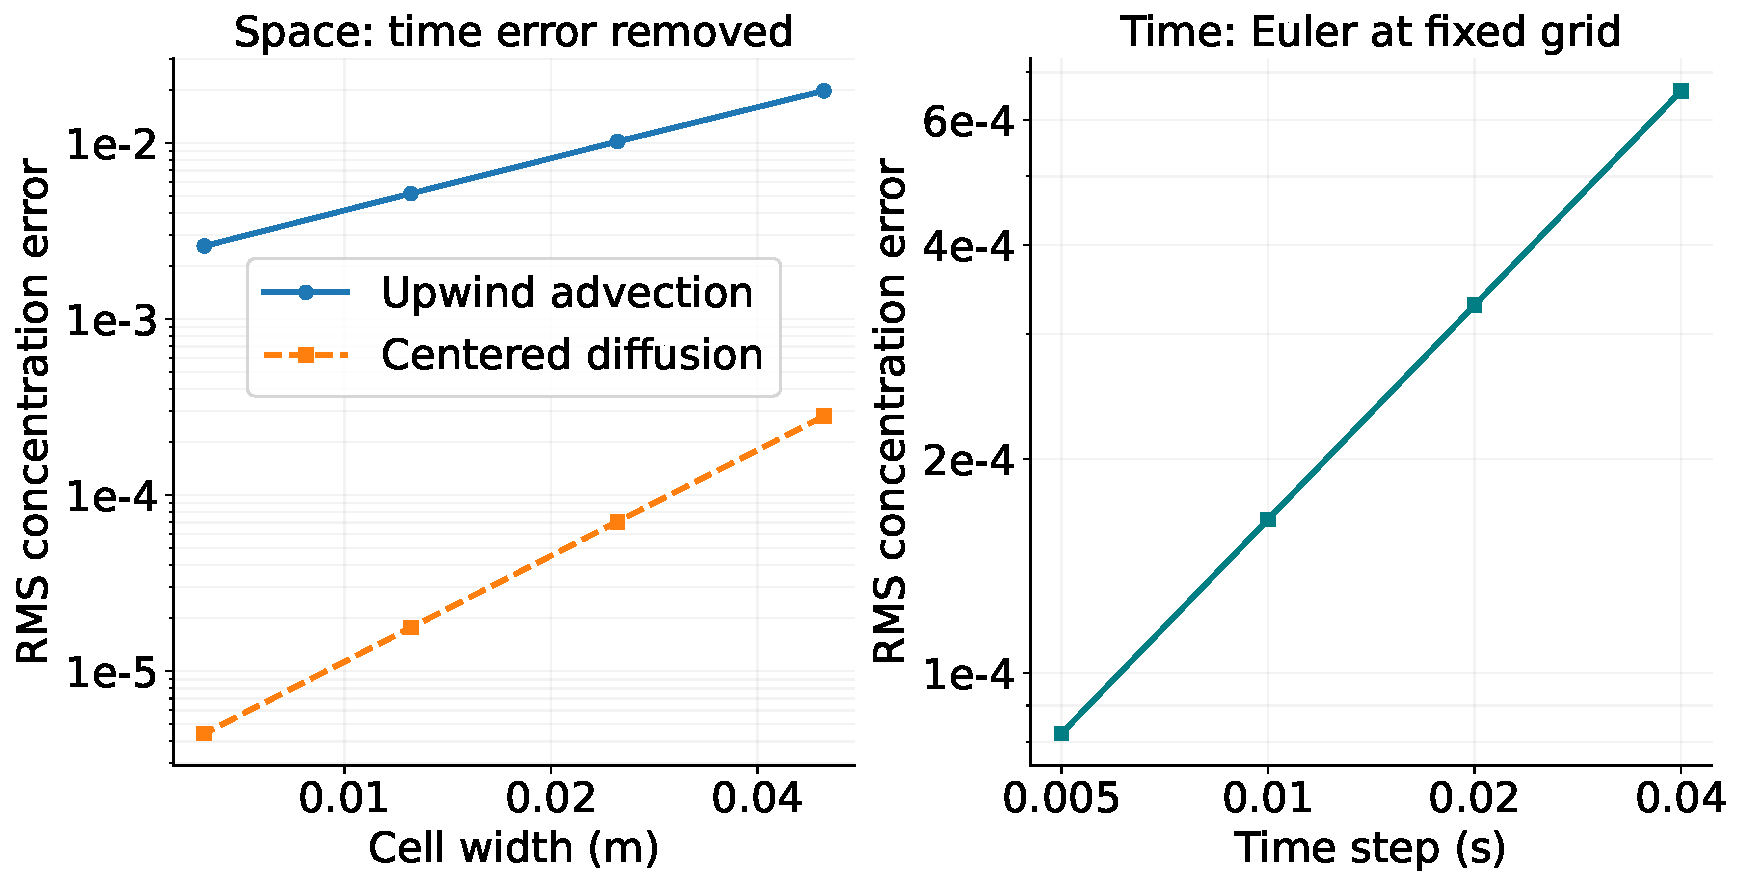
\includegraphics[width=.96\linewidth,height=.57\textheight,keepaspectratio]{separate-errors.pdf}\par\smallskip
{\small Exact single-mode references isolate spatial error and Euler time error. The two panels vary different numerical controls and use different references.}
\end{minipage}\end{center}
\section{Separate space and time refinement}
\hypertarget{note-separate-space-and-time-refinement}{}\label{note:separate-space-and-time-refinement}
{\small \href{slides.html\#frame=euler-amplification-at-a-fixed-grid\&step=1}{Slides for this section} \quad \href{../modules/cfd/index.html}{Conservation, viscous flow and transport}}\par
The original spatial experiment uses 20, 40, 80 and 160 cells at a final time of 0.5 s. It separates pure advection with a=0.2 m/s from pure diffusion with D=0.01 m\ensuremath{^{2}}/s. For the upwind case, the successive observed orders are approximately 0.958, 0.981 and 0.991. For centered diffusion they are approximately 1.993, 1.998 and 2.000. These are computed results of the supplied code and chosen reference, not values copied from a textbook plot.

The temporal experiment fixes 64 cells, a=0.1 m/s, D=0.001 m\ensuremath{^{2}}/s and final time 0.4 s. Steps of 0.04, 0.02, 0.01 and 0.005 s all meet the explicit positivity bound. Their errors relative to exact semi-discrete evolution are approximately 6.59\ensuremath{\times}10\ensuremath{^{-4}}, 3.29\ensuremath{\times}10\ensuremath{^{-4}}, 1.64\ensuremath{\times}10\ensuremath{^{-4}} and 8.22\ensuremath{\times}10\ensuremath{^{-5}}. The error nearly halves each time, consistent with first-order Euler time stepping.

For $N_t=T/\Delta t$ equal steps, the numerical modal amplitude is
\[
 z^{N_t}=(1+\Delta t\lambda_h)^{N_t}z^0.
\]
Its logarithm is $T\lambda_h-\tfrac12T\Delta t\lambda_h^2+O(\Delta t^2)$ at fixed grid. Comparing with $e^{T\lambda_h}z^0$ isolates the first-order temporal contribution without changing the spatial operator.
\section{The highest-frequency diffusion mode}
\hypertarget{note-the-highest-frequency-diffusion-mode}{}\label{note:the-highest-frequency-diffusion-mode}
{\small \href{slides.html\#frame=a-grid-scale-perturbation\&step=1}{Slides for this section} \quad \href{../modules/cfd/index.html}{Conservation, viscous flow and transport}}\par
The smooth sine is a useful accuracy benchmark but a poor stress test for the smallest resolvable scales. Consider an alternating-cell perturbation, positive in one cell and negative in the next, around a uniform mean. For pure diffusion the centered second difference multiplies this perturbation by minus four divided by spacing squared. One Euler step therefore multiplies its amplitude by 1\ensuremath{-}4\ensuremath{\mu}, where \ensuremath{\mu}=D\ensuremath{\Delta}t/\ensuremath{\Delta}x\ensuremath{^{2}}.

At \ensuremath{\mu}=0.4 the amplification is \ensuremath{-}0.6: the perturbation changes sign while its magnitude shrinks. At \ensuremath{\mu}=0.6 the amplification is \ensuremath{-}1.4: it changes sign and grows by a factor of 1.4 per step. The alternating perturbation still sums to zero, so its growth can leave the total amount exactly conserved. Eventually concentrations can become negative or excessively large even though a mass check continues to pass.

The unstable curve in the figure is an analytic amplification diagnostic. The production solver rejects that parameter choice instead of silently running it. This distinction matters: a deliberate counterexample belongs in a labeled experiment, while the ordinary solver should fail clearly when a requested setting violates its stated admissibility condition. The full symbol above supplies the amplification at every resolved spatial wave number.

\[
\epsilon^{n+1}=(1-4\mu)\epsilon^n,\qquad \mu=D\Delta t/\Delta x^2
\]
Its magnitude grows when \ensuremath{\mu}>1/2. The total perturbation remains zero on an even periodic grid.

At $\theta=\pi$, the alternating mode has zero discrete mean and diffusion eigenvalue $-4D/\Delta x^2$. Thus conservation of its mean is compatible with unbounded growth in its amplitude. The condition $|1-4\mu|\le1$ gives $0\le\mu\le1/2$, precisely the pure-diffusion restriction obtained from nonnegative stencil weights.
\begin{center}\begin{minipage}{.98\linewidth}\centering
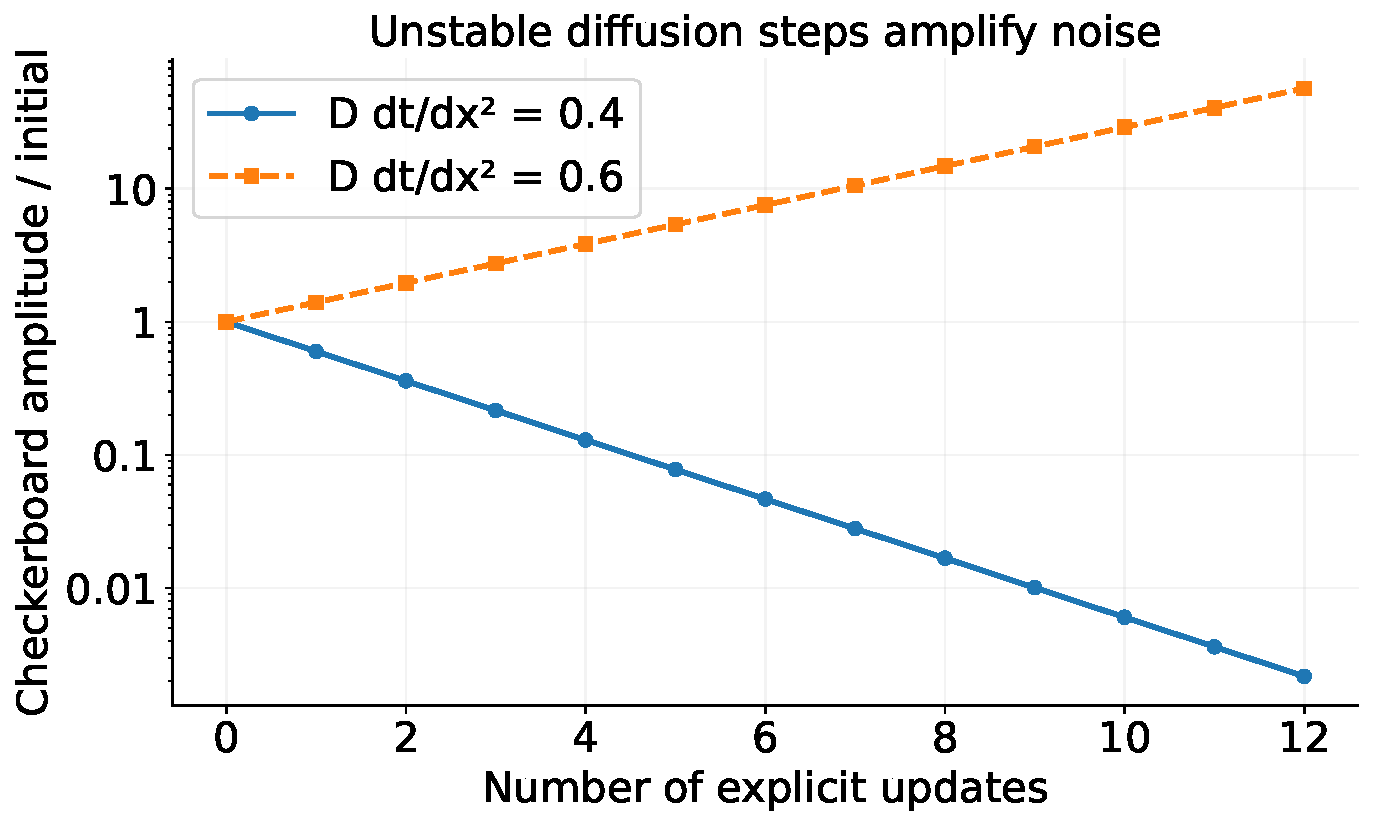
\includegraphics[width=.96\linewidth,height=.57\textheight,keepaspectratio]{stability-mode.pdf}\par\smallskip
{\small The plotted amplification is an analytic checkerboard diagnostic. The executable solver rejects the unstable $\mu$=\allowbreak{}0.6 setting.}
\end{minipage}\end{center}
\section{Limits of the single-mode analysis}
\hypertarget{note-limits-of-the-single-mode-analysis}{}\label{note:limits-of-the-single-mode-analysis}
{\small \href{slides.html\#frame=the-scope-of-fourier-analysis\&step=1}{Slides for this section} \quad \href{../modules/cfd/index.html}{Conservation, viscous flow and transport}}\par
Those results do not certify every initial condition or boundary implementation, and they do not validate a physiological model. A discontinuous pulse may converge differently in a chosen norm. A new boundary condition can introduce a new error source. Before reusing the solver in a more complex project, add tests targeted at the added features. Each added feature requires an appropriate reference or limiting calculation.

Fourier diagonalization applies here because the coefficients are constant and the grid is periodic. New boundaries, variable coefficients, discontinuities or nonlinear reactions remove some of this structure. The single-mode calculation identifies the behavior of the present operator; it is not a theorem about every extension using the same time loop.
\bigskip
\section*{Exercises}
\par\noindent\begin{minipage}{\linewidth}
\subsection*{E1. Interpret an order table}
At spacings 0.08, 0.04 and 0.02 m, a fixed-time benchmark gives RMS errors 0.0128, 0.0032 and 0.0008.

\textbf{a} Compute the two observed orders.

\end{minipage}\par\medskip
\textbf{b} Under the same asymptotic law, estimate the error at 0.01 m.

\textbf{c} Would this table validate a patient-flow prediction?

\par\noindent\begin{minipage}{\linewidth}
\subsection*{E2. Separate two error sources}
Suppose the leading error estimate is E$\approx$2h+\allowbreak{}5$\Delta$t, with dimensionless h and $\Delta$t for this exercise.

\textbf{a} Compute E for (h,$\Delta$t)=\allowbreak{}(0.04,0.01), then for (0.02,0.005).

\end{minipage}\par\medskip
\textbf{b} Does the ratio alone identify the spatial coefficient or temporal coefficient?

\textbf{c} Design two experiments that separate the errors.

\par\noindent\begin{minipage}{\linewidth}
\subsection*{E3. An unstable but conservative perturbation}
On an even periodic grid use pure diffusion with $\mu$=\allowbreak{}0.55 and an alternating perturbation of amplitude 0.01 around mean one.

\textbf{a} Find the amplification and the amplitude after three steps.

\end{minipage}\par\medskip
\textbf{b} What happens to the total amount and what does that show?

\textbf{c} What should the ordinary solver do with this setting?

\par\noindent\begin{minipage}{\linewidth}
\subsection*{E4. Match the reference state}
Let c(x)=\allowbreak{}1+\allowbreak{}0.3 sin(2$\pi$x/L) with L=\allowbreak{}1 m and cells of width 0.1 m.

\textbf{a} Write the exact cell-average amplitude factor and estimate it.

\end{minipage}\par\medskip
\textbf{b} Why could a midpoint comparison disguise another second-order error?

\section*{References}
\noindent\begin{minipage}{\linewidth}
Zan Ahmad, Advanced Topics in Computational Cardiology syllabus, Fall 2024. PDF pages 1--2.

\end{minipage}\par\medskip
\noindent\begin{minipage}{\linewidth}
Hoppensteadt and Peskin, Modeling and Simulation in Medicine and the Life Sciences, second edition. Printed page 317; supplied PDF page 327 (diffusion scaling and continuum limit).

\end{minipage}\par\medskip
\noindent\begin{minipage}{\linewidth}
NASA NPARC Alliance, Examining Spatial (Grid) Convergence. Introduction; Order of Grid Convergence; Asymptotic Range of Convergence.

\url{https://www.grc.nasa.gov/www/wind/valid/tutorial/spatconv.html}
\end{minipage}\par\medskip
\end{document}
